\begin{frame}
\frametitle{Tabela de conteúdos}
\tableofcontents
\end{frame}

% ------------------------------------------
% ------------------------------------------

\section{Introdução}

\begin{frame}
  \frametitle{Objetivo da reconstrução 3D}

  \underline{Inferir} a geometria e a estrutura de objetos e cenas.

\end{frame}

% ------------------------------------------
% ------------------------------------------

\begin{frame}
  \frametitle{Aplicações}
\begin{itemize}
  \item como navegação por robô;
  \item reconhecimento de objetos e compreensão de cenas;
  \item modelagem 3D e animação;
  \item controle industrial;
  \item diagnóstico médico
\end{itemize}

\end{frame}

% ------------------------------------------
% ------------------------------------------

\begin{frame}
  \frametitle{sistema estereoscópico}
A recuperação da dimensão perdida a partir de apenas imagens 2D foi o objetivo
do estéreo multivista clássico, que foi extensivamente investigado por
muitas décadas.

A primeira geração de métodos abordava o problema da perspectiva geométrica;
eles focavam na compreensão e formalização, matematicamente, do 3D ao
processo de projeção 2D, com o objetivo de elaborar soluções técnicas ou
algorítmicas.

\end{frame}

% ------------------------------------------
\begin{frame}
  \frametitle{sistema estereoscópico}
\begin{figure}[h!]
  \begin{center}
    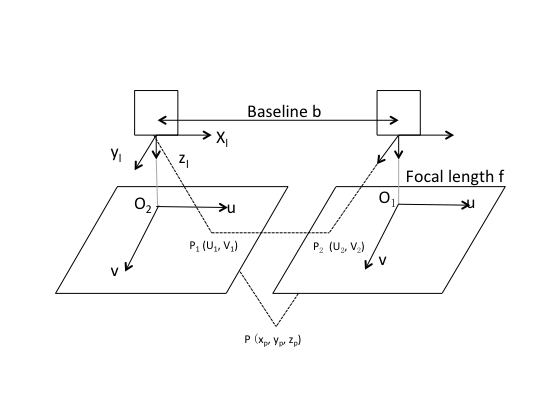
\includegraphics[width=\textwidth]{images/Stereoscopic_schematic.png}
  \end{center}
  \caption{Geometria de um sistema estereoscópico}
  \label{fig:7-40}
\end{figure}

\end{frame}

% ------------------------------------------
% ------------------------------------------
\begin{frame}
  \frametitle{Lei de Gauss}

Método deterministico

\begin{alertblock}{ relacionamos áreas com volume }

\[ \iint_{\partial s} \overrightarrow{F}\cdot \overrightarrow{n}ds
  = \iiint_{W}\nabla\cdot\overrightarrow{F} dxdydz \]

\end{alertblock}

\end{frame}
\end{frame}
% ------------------------------------------
% ------------------------------------------

% ------------------------------------------
\begin{frame}
  \frametitle{Objetivo da reconstrução 3D}

\begin{alertblock}{Eulerian equations of ideal magnetohydrodynamics (MHD)
including    gravity, in comoving coordinate}
\[ \frac{\partial \rho }{\partial t} + \frac{1}{a}\nabla .(\rho \vec{v}) =
    0
\]
\[ \frac{\partial \rho \vec{v}}{\partial t} + \dfrac{1}{a}\nabla
    .\left(\rho \vec{v}\vec{v} + \vec{I}p^* - \frac{\vec{B}\vec{B}}{a}\right) =
    -\frac{\dot{a}}{a}\rho \vec{v} - \frac{1}{a}\rho \nabla \phi
\]
    \begin{alignat*}{2}
      \frac {\partial E} {\partial t} + \frac {1}{a} \nabla . \left[ (E+p^*) -
        \frac{1}{a}\vec{B}(\vec{B}.\vec{v})\right] &= &&-
      \frac{\dot{a}}{a}\left(2E - \frac{B^2}{2a}\right) \\
      & &&  - \frac{\rho}{a}\vec{v}.\nabla \phi
      - \Lambda + \Gamma\\
      & && + \dfrac{1}{a^2}\nabla . \vec{F}_{cond},
    \end{alignat*}

\end{alertblock}

\end{frame}

% ------------------------------------------
% ------------------------------------------
\frame{dummy frame}
